%!TEX root = modelguide.tex

\chapter{Simulation Control}
\label{SimulationControl:sec}

This section describes different devices which an application may use
to control the simulation. These include {\it control panels} to allow
for the interactive adjustment of properties, as well as {\it agents}
which are applied every time step. Agents include {\it controllers}
and {\it input probes} to supply and modify input parameters at the
beginning of each time step, and {\it monitors} and {\it output
probes} to observe and record simulation results at the end of each
time step.

\section{Control Panels}
\label{ControlPanels:sec}

A {\it control panel} is an editing panel that allows for the
interactive adjustment of component properties.

It is always possible to adjust component properties through the GUI
by selecting one or more components and then choosing {\sf Edit
properties ...} in the right-click context menu. However, it may be
tedious to repeatedly select the required components, and the
resulting panels present the user with {\it all} properties common to
the selection.  A control panel allows an application to provide a
customized editing panel for selected properties.

\subsection{General principles}

Control panels are implemented by the
\javaclass[artisynth.core.gui]{ControlPanel} model component.  They
can be set up within a model's {\tt build()} method by creating an
instance of {\tt ControlPanel}, populating it with widgets for editing
the desired properties, and then adding it to the root model using the
latter's
\javamethod*[artisynth.core.workspace.RootModel]{addControlPanel()}
method.

One of the most commonly used means of adding widgets to a control
panel is the method
\javamethodAlt{artisynth.core.gui.ControlPanel.addWidget(HasProperties,String)}%
{addWidget(comp,propertyPath)}, which creates a widget for a property
specified by {\tt propertyPath} with respect to the component
{\tt comp}.  Property paths are discussed in the Section
\ref{PropertyHandlesAndPaths:sec}, and can consist solely of a
property name, or, for properties located in descendant components, a
component path followed by a colon `{\tt :}' and the property name.

Other flavors of {\tt addWidget()} also exist, as described in the API
documentation for \javaclass[artisynth.core.gui]{ControlPanel}.  In
addition to property widgets, any type of {\tt Swing} or {\tt awt}
component can be added using the method
\javamethodAlt{artisynth.core.gui.ControlPanel.addWidget(Component)}%
{addWidget(awtcomp)}.

Control panels can also be created interactively using the GUI; see
the section ``Control Panels'' in the
\href{\artisynthDocBase/html/uiguide/uiguide.html}{
ArtiSynth User Interface Guide}.

\subsection{Example: Creating a simple control panel}

\begin{figure}[t]
\begin{center}
\iflatexml
 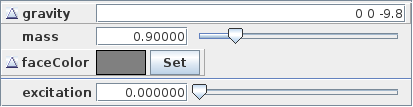
\includegraphics[]{images/controlPanel}
\else
 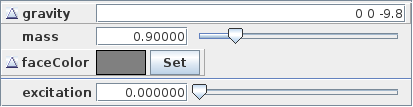
\includegraphics[width=3in]{images/controlPanel}
\fi
\end{center}
\caption{Control panel created by the model {\tt SimpleMuscleWithPanel}.}
\label{controlPanel:fig}
\end{figure}

An application model showing a control panel is defined in
%
\begin{verbatim}
  artisynth.demos.tutorial.SimpleMuscleWithPanel
\end{verbatim}
%
This model simply extends {\tt SimpleMuscle} (Section
\ref{SimpleMuscleExample:sec}) to provide a control panel for
adjusting gravity, the mass and color of the box, and the muscle
excitation. The class definition, excluding {\tt include} statements,
is shown below:
%
\lstset{numbers=left}
\begin{lstlisting}[]
public class SimpleMuscleWithPanel extends SimpleMuscle {
   ControlPanel panel;

   public void build (String[] args) throws IOException {

      super.build (args);

      // add control panel for gravity, rigod body mass and color, and excitation
      panel = new ControlPanel("controls");
      panel.addWidget (mech, "gravity");
      panel.addWidget (mech, "rigidBodies/box:mass");
      panel.addWidget (mech, "rigidBodies/box:renderProps.faceColor");
      panel.addWidget (new JSeparator());
      panel.addWidget (muscle, "excitation");

      addControlPanel (panel);
   }
}
\end{lstlisting}
\lstset{numbers=none}
%
The {\tt build()} method calls {\tt super.build()} to create the model
used by {\tt SimpleMuscle}. It then proceeds to create a {\tt
ControlPanel}, populate it with widgets, and add
it to the root model (lines 8-15). The panel is given the name {\tt
"controls"} in the constructor (line 8); this is its component name
and is also used as the title for the panel's window frame. A control
panel does not need to be named, but if it is, then that name must be
unique among the control panels.

Lines 9-11 create widgets for three properties located relative to the
{\tt MechModel} referenced by {\tt mech}. The first is the {\tt
MechModel}'s {\tt gravity}. The second is the {\tt mass} of the box,
which is a component located relative to {\tt mech} by the path name
(Section \ref{PathNames:sec}) {\tt "rigidBodies/box"}. The third is
the box's face color, which is the sub-property {\tt faceColor} of the
box's {\tt renderProps} property.

Line 12 adds a {\tt JSeparator} to the panel, using the {\tt
addWidget()} method that accepts general components, and line 13 adds
a widget to control the {\tt excitation} property for {\tt muscle}.

\begin{sideblock}
It should be noted that there are different ways to specify target
properties in {\tt addWidget()}. First, component paths may contain
numbers instead of names, and so the box's mass property could be
specified using {\tt "rigidBodies/0:mass"} instead of {\tt
"rigidBodies/box:mass"} since the box's number is 0. Second, if a
reference to a sub-component is available, one can specify properties
directly with respect to that, instead of indicating the sub-component
in the property path. For example, if the box was referenced by a
variable {\tt body}, then one could use the construction
%
\begin{verbatim}
   panel.addWidget (body, "mass");
\end{verbatim}
%
in place of 
%
\begin{verbatim}
   panel.addWidget (mech, "rigidBodies/box:mass");
\end{verbatim}
%
\end{sideblock}

To run this example in ArtiSynth, select {\sf All demos > tutorial >
SimpleMuscleWithPanel} from the {\sf Models} menu. The properties 
shown in the panel can be adjusted interactively by the user,
while the model is either stationary or running.
% SimpleMuscleWithPanel

\section{Custom properties}
\label{CustomProperties:sec}

Because of the usefulness of properties in creating control panels and
probes (Sections \ref{ControlPanels:sec}) and Section
\ref{Probes:sec}), model developers may wish to add their own
properties, either to the root model, or to a custom component.

This section provides only a brief summary of how to define
properties. Full details are available in the ``Properties'' section of
the \href{\artisynthDocBase/html/maspack/maspack.html}{
Maspack Reference Manual}.

\subsection{Adding properties to a component}

As mentioned in Section \ref{Properties:sec}, properties are
class-specific, and are exported by a class through code contained in
the class's definition.  Often, it is convenient to add properties to
the {\tt RootModel} subclass that defines the application model. In
more advanced applications, developers may want to add properties to a
custom component.

The property definition steps are:

\begin{description}

\item[Declare the property list:]\mbox{}

The class exporting the properties creates its own static instance of
a \javaclass[maspack.properties]{PropertyList}, using a declaration
like
%
\begin{lstlisting}[]
   static PropertyList myProps = new PropertyList (MyClass.class, MyParent.class);

   @Override   
   public PropertyList getAllPropertyInfo() {
      return myProps;
   }  
\end{lstlisting}
%
where {\tt MyClass} and {\tt MyParent} specify the class types of the
exporting class and its parent class. The {\tt PropertyList}
declaration creates a new property list, with a copy of all the
properties contained in the parent class.  If one does {\it not} want
the parent class properties, or if the parent class does not have
properties, then one would use the constructor
\javamethodAlt{maspack.properties.PropertyList.PropertyList(Class)}%
{PropertyList(MyClass.class)} instead. If the parent class is an
ArtiSynth model component (including the {\tt RootModel}), then it
will always have its own properties. The declaration of the method
{\tt getAllPropertyInfo()} exposes the property list to other classes.

\item[Add properties to the list:]\mbox{}

Properties can then be added to the property list, by calling the {\tt
PropertyList}'s
\javamethod*[maspack.properties.PropertyList]{add(String,String,Object)}
method:
%
\begin{lstlisting}[]
   PropertyDesc add (String name, String description, Object defaultValue);
\end{lstlisting}
%
where {\tt name} contains the name of the property, {\tt description}
is a comment describing the property, and {\tt defaultValue} is an
object containing the property's default value.  This is done inside a
static code block:
%
\begin{lstlisting}[]
   static {
      myProps.add ("stiffness", "spring stiffness", /*defaultValue=*/1);
      myProps.add ("damping", "spring damping", /*defaultValue=*/0);
   }
\end{lstlisting}
%
Variations on the {\tt add()} method exist for adding {\it read-only}
or {\it inheritable} properties, or for setting various property
options. Other methods allow the property list to be edited.

\item[Declare property accessor functions:]\mbox{}

For each property {\tt propXXX} added to the property list, accessor methods of
the form
%
\begin{lstlisting}[]
   void setPropXXX (TypeX value) {
      ...
   }

   TypeX getPropXXX() {
      TypeX value = ...
      return value;
   }
\end{lstlisting}
%
must be declared, where {\tt TypeX} is the value associated with the
property. 
\begin{sideblock}
It is possible to specify different names for the accessor functions
in the string argument {\tt name} supplied to the {\tt add()}
method. Read-only properties only require a {\it get} accessor.
\end{sideblock}

\end{description}

\subsection{Example: a visibility property}
%
An model illustrating the exporting of properties is defined in
%
\begin{verbatim}
  artisynth.demos.tutorial.SimpleMuscleWithProperties
\end{verbatim}
%
This model extends {\tt SimpleMuscleWithPanel} (Section
\ref{SimpleMuscleExample:sec}) to provide a custom property
{\tt boxVisible} that is added to the control panel.
The class definition, excluding {\tt include} statements,
is shown below:
%
\lstset{numbers=left}
\begin{lstlisting}[]
public class SimpleMuscleWithProperties extends SimpleMuscleWithPanel {

   // internal property list; inherits properties from SimpleMuscleWithPanel
   static PropertyList myProps =
      new PropertyList (
         SimpleMuscleWithProperties.class, SimpleMuscleWithPanel.class);

   // override getAllPropertyInfo() to return property list for this class
   public PropertyList getAllPropertyInfo() {
      return myProps;
   }

   // add new properties to the list
   static {
      myProps.add ("boxVisible", "box is visible", false);
   }

   // declare property accessors
   public boolean getBoxVisible() {
      return box.getRenderProps().isVisible();
   }

   public void setBoxVisible (boolean visible) {
      RenderProps.setVisible (box, visible);
   }

   public void build (String[] args) throws IOException {

      super.build (args);

      panel.addWidget (this, "boxVisible");
      panel.pack();
   }
}
\end{lstlisting}
\lstset{numbers=none}
%
First, a property list is created for the application class {\tt
SimpleMuscleWithProperties.class} which contains a copy of all the
properties from the parent class {\tt SimpleMuscleWithPanel.class}
(lines 4-6). This property list is made visible by overriding {\tt
getAllPropertyInfo()} (lines 9-11). The {\tt boxVisible} property
itself is then added to the property list (line 15), and accessor
functions for it are declared (lines 19-25).

\begin{figure}[t]
\begin{center}
\iflatexml
 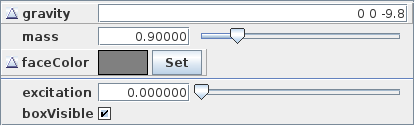
\includegraphics[]{images/boxVisiblePanel}
\else
 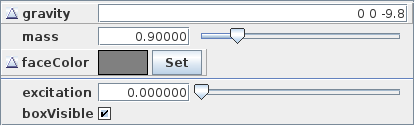
\includegraphics[width=3in]{images/boxVisiblePanel}
\fi
\end{center}
\caption{Control panel created by the model {\tt SimpleMuscleWithProperties},
showing the newly defined property {\tt boxVisible}.}
\label{boxVisiblePanel:fig}
\end{figure}

The {\tt build()} method calls {\tt super.build()} to perform all the
model creation required by the super class, and then adds an
additional widget for the {\tt boxVisible} property to the control
panel.

To run this example in ArtiSynth, select {\sf All demos > tutorial >
SimpleMuscleWithProperties} from the {\sf Models} menu. The control
panel will now contain an additional widget for the property {\tt
boxVisible} as shown in Figure \ref{boxVisiblePanel:fig}. Toggling
this property will make the box visible or invisible in the viewer.

% SimpleMuscleWithProperties

\section{Controllers and monitors}
\label{ControllersAndMonitors:sec}

Application models can define custom {\it controllers} and {\it
monitors} to control input values and monitor output values as a
simulation progresses. Controllers are called every time step
immediately before the {\tt advance()} method, and monitors are called
immediately after (Section \ref{ModelAdvancement:sec}).  An example of
controller usage is provided by ArtiSynth's inverse modeling feature,
which uses an internal controller to estimate the actuation signals
required to follow a specified motion trajectory.

More precise details about controllers and monitors and how they
interact with model advancement are given in the
\href{\artisynthDocBase/html/artisynth/artisynth.html}{
ArtiSynth Reference Manual}.

\subsection{Implementation}
\label{ControllerImplementation:sec}

Applications may declare whatever controllers or monitors they require
and then add them to the root model using the methods
\javamethod*[artisynth.core.workspace.RootModel]{addController()} and
\javamethod*[artisynth.core.workspace.RootModel]{addMonitor()}.
They can be any type of
\javaclass[artisynth.core.modelbase]{ModelComponent} that implements
the \javaclass[artisynth.core.modelbase]{Controller} or
\javaclass[artisynth.core.modelbase]{Monitor} interfaces.  For
convenience, most applications simply subclass
the default implementations
\javaclass[artisynth.core.modelbase]{ControllerBase} or
\javaclass[artisynth.core.modelbase]{MonitorBase} and then override
the necessary methods.

The primary methods associated with both controllers and
monitors are:
%
\begin{lstlisting}[]
  public void initialize (double t0);

  public void apply (double t0, double t1);

  public boolean isActive();
\end{lstlisting}
%
{\tt apply(t0, t1)} is the ``business'' method and is called once per
time step, with {\tt t0} and {\tt t1} indicating the start and end
times $t_0$ and $t_1$ associated with the step.  {\tt initialize(t0)}
is called whenever an application model's state is set (or reset) at a
particular time $t_0$. This occurs when a simulation is first started
or after it is reset (with $t_0 = 0$), and also when the state is
reset at a waypoint or during adaptive stepping.

{\tt isActive()} controls whether a controller or monitor is active;
if {\tt isActive()} returns {\tt false} then the {\tt apply()} method
will not be called.
The default implementations
\javaclass[artisynth.core.modelbase]{ControllerBase} and
\javaclass[artisynth.core.modelbase]{MonitorBase}, via their
superclass \javaclass[artisynth.core.modelbase]{ModelAgentBase}, also
provide a {\tt setActive()} method to control this setting, and export
it as the property {\sf active}. This allows controller and monitor
activity to be controlled at run time.

\begin{sideblock}
To enable or disable a controller or monitor at run time, locate it in
the navigation panel (under the RootModel's {\sf controllers} or {\sf
monitors} list), chose {\sf Edit properties ...} from the right-click
context menu, and set the {\sf active} property as desired.
\end{sideblock}

Controllers and monitors may be associated with a particular model
(among the list of models owned by the root model). This model may be
set or queried using
%
\begin{lstlisting}[]
  void setModel (Model m);

  Model getModel();
\end{lstlisting}
%
If associated with a model, {\tt apply()} will be called immediately
before (for controllers) or after (for monitors) the model's {\tt
advance()} method. If not associated with a model, then {\tt apply()}
will be called before or after the advance of {\it all} the models
owned by the root model.

Controllers and monitors may also contain {\it state}, in which case
they should implement the relevant methods from the
\javaclass[artisynth.core.modelbase]{HasState} interface.

Typical actions for a controller include setting input forces or
excitation values on components, or specifying the motion trajectory
of parametric components (Section \ref{DynamicVsParametric:sec}).
Typical actions for a monitor include observing or recording
the motion profiles or constraint forces that arise
from the simulation.

When setting the position and/or velocity of a dynamic component that
has been set to be parametric (Section \ref{DynamicVsParametric:sec}),
a controller should not set its position or velocity directly, but
should instead set its {\it target position} and/or {\it target
velocity}, since this allows the solver to properly interpolate the
position and velocity during the time step. The methods to set or
query target positions and velocities for
\javaclass[artisynth.core.mechmodels]{Point}-based components are
%
\begin{lstlisting}[]
  setTargetPosition (Point3d pos);
  Point3d getTargetPosition ();       // read-only

  setTargetVelocity (Vector3d vel);
  Vector3d getTargetVelocity ();      // read-only
\end{lstlisting}
%
while for
\javaclass[artisynth.core.mechmodels]{Frame}-based components they are
%
\begin{lstlisting}[]
  setTargetPosition (Point3d pos);
  setTargetOrientation (AxisAngle axisAng);
  setTargetPose (RigidTransform3d TFW);
  Point3d getTargetPosition ();       // read-only
  AxisAngle getTargetOrientation ();  // read-only
  RigidTransform3d getTargetPose();   // read-only

  setTargetVelocity (Twist vel);
  Twist getTargetVelocity ();         // read-only
\end{lstlisting}
%

\subsection{Example: A controller to move a point}

A model showing an application-defined controller is defined in
%
\begin{verbatim}
  artisynth.demos.tutorial.SimpleMuscleWithController
\end{verbatim}
%
This simply extends {\tt SimpleMuscle} (Section
\ref{SimpleMuscleExample:sec}) and adds a controller which moves the
fixed particle {\tt p1} along a circular path.  The complete class
definition is shown below:
%
\lstset{numbers=left}
\lstinputlisting{../../src/artisynth/demos/tutorial/SimpleMuscleWithController.java}
\lstset{numbers=none}
%
A controller called {\tt PointMover} is defined by extending {\tt
ControllerBase} and overriding the {\tt apply()} method. It stores the
point to be moved in {\tt myPnt}, and the initial position in
{\tt myPos0}. The {\tt apply()} method computes a target position for
the point that starts at {\tt myPos0} and then moves in a circle in the
$x-z$ plane with an angular velocity of $\pi/2$ rad/sec (lines 22-28).

The {\tt build()} method calls {\tt super.build()} to create the model
used by {\tt SimpleMuscle}, and then creates an instance of {\tt
PointMover} to move particle {\tt p1} and adds it to the root model
(line 34). The viewer bounds are updated to make the circular motion
more visible (line 36).

To run this example in ArtiSynth, select {\sf All demos > tutorial >
SimpleMuscleWithController} from the {\sf Models} menu. When
the model is run, the fixed particle {\tt p1} will trace
out a circular path in the $x-z$ plane.

\section{Probes}
\label{Probes:sec}

In addition to controllers and monitors, applications can also attach
streams of data, known as {\it probes}, to input and output values
associated with the simulation. Probes derive from the same base class
\javaclass[artisynth.core.modelbase]{ModelAgentBase} as 
controllers and monitors, 
but differ in that 

\begin{enumerate}

\item They are associated with an explicit time interval during which
they are applied;

\item They can have an attached file for supplying input data or
recording output data;

\item They are displayable in the ArtiSynth {\it timeline} panel.

\end{enumerate}

A probe is applied (by calling its {\tt apply()} method) only for time
steps that fall within its time interval. This interval can be set and
queried using the following methods:
%
\begin{lstlisting}[]
   setStartTime (double t0);
   setStopTime (double t1);
   setInterval (double t0, double t1);
 
   double getStartTime();
   double getStopTime();
\end{lstlisting}
%
The probe's attached file can be set and queried using:
%
\begin{lstlisting}[]
   setAttachedFileName (String fileName);
   String getAttachedFileName ();
\end{lstlisting}
%
where {\tt fileName} is a string giving the file's path name.

Details about the timeline display can be found in
the section ``The Timeline'' in the
\href{\artisynthDocBase/html/uiguide/uiguide.html}{
ArtiSynth User Interface Guide}.

There are two types of probe: {\it input probes}, which are applied at
the beginning of each simulation step before the controllers, and {\it
output probes}, which are applied at the end of the step after the
monitors.

While applications are free to construct any type of probe by
subclassing either \javaclass[artisynth.core.probes]{InputProbe} or
\javaclass[artisynth.core.probes]{OutputProbe}, most applications
utilize either \javaclass[artisynth.core.probes]{NumericInputProbe} or
\javaclass[artisynth.core.probes]{NumericOutputProbe}, which
explicitly implement streams of numeric data which are connected to
properties of various model components.  The remainder of this section
will focus on numeric probes.

As with controllers and monitors, probes also implement a {\tt
isActive()} method that indicates whether or not the probe is active.
Probes that are not active are not invoked. Probes also provide a
{\tt setActive()} method to control this setting, and export it as the
property {\sf active}. This allows probe activity to be controlled at
run time.

\begin{sideblock}
To enable or disable a probe at run time, locate it in the navigation
panel (under the RootModel's {\sf inputProbes} or {\sf outputProbes}
list), chose {\sf Edit properties ...} from the right-click context
menu, and set the {\sf active} property as desired.

Probes can also be enabled or disabled in the timeline, by either
selecting the probe and invoking {\sf activate} or {\sf deactivate}
from the right-click context menu, or by clicking the track {\sf mute}
button (which activates or deactivates all probes on that track).
\end{sideblock}

\subsection{Numeric probe structure}
\label{NumericProbeStructure:sec}

Numeric probes are associated with:

\begin{itemize}

\item {\it A vector of temporally-interpolated numeric data};

\item {\it One or more properties} to which the probe is bound and
which are either set by the numeric data (input probes), or used to
set the numeric data (output probes).

\end{itemize}

The numeric data is implemented internally by a
\javaclass[maspack.interpolation]{NumericList}, which stores the data
as a series of vector-valued knot points at prescribed times $t_k$ and
then interpolates the data for an arbitrary time $t$ using an
interpolation scheme provided by
\javaclass[maspack.interpolation]{Interpolation}.

Some of the numeric probe methods associated with the interpolated
data include:
%
\begin{lstlisting}[]
   int getVsize();                      // returns the size of the data vector
   setInterpolationOrder (Order order); // sets the interpolation scheme
   Order getInterpolationOrder();       // returns the interpolation scheme

   VectorNd getData (double t);         // interpolates data for time t
   NumericList getNumericList();        // returns the underlying NumericList
\end{lstlisting}
%
Interpolation schemes are described by the enumerated type {\tt
Interpolation.Order} and presently include:

\begin{description}

\item[Step]\mbox{}

Values at time $t$ are set to the values of the closest knot point
$k$ such that $t_k \le t$.

\item[Linear]\mbox{}

Values at time $t$ are set by linear interpolation of the knot points
$(k, k+1)$ such that $t_k \le t \le t_{k+1}$.

\item[Parabolic]\mbox{}

Values at time $t$ are set by quadratic interpolation of the knots
$(k-1, k, k+1)$ such that $t_k \le t \le t_{k+1}$.

\item[Cubic]\mbox{}

Values at time $t$ are set by cubic Catmull interpolation of the knots
$(k-1, \ldots, k+2)$ such that $t_k \le t \le t_{k+1}$.

\end{description}

Each property bound to a numeric probe must have a value
that can be mapped onto a scalar or vector value. Such properties
are know as {\it numeric properties}, and whether or not
a value is numeric can be tested
using \javamethodAlt{maspack.properties.NumericConverter.isNumeric()}%
{NumericConverter.isNumeric(value)}.

By default, the total number of scalar and vector values associated
with all the properties should equal the size of the interpolated
vector (as returned by
\javamethod*[artisynth.core.probes.NumericProbeBase]{getVsize()}).
However, it is possible to establish more complex mappings between the
property values and the interpolated vector. These mappings are beyond
the scope of this document, but are discussed in the sections ``General
input probes'' and ``General output probes'' of the
\href{\artisynthDocBase/html/uiguide/uiguide.html}{
ArtiSynth User Interface Guide}.

\subsection{Creating probes in code}

This section discusses how to create numeric probes in code.  They can
also be created and added to a model graphically, as described in the
section ``Adding and Editing Numeric Probes'' in the
\href{\artisynthDocBase/html/uiguide/uiguide.html}{
ArtiSynth User Interface Guide}.

Numeric probes have a number of constructors and methods that make it
relatively easy to create instances of them in code. For 
\javaclass[artisynth.core.probes]{NumericInputProbe}, there
is the constructor
%
\begin{lstlisting}[]
   NumericInputProbe (ModelComponent c, String propPath, String filePath);
\end{lstlisting}
%
which creates a {\tt NumericInputProbe}, binds it to a property
located relative to the component {\tt c} by {\tt propPath}, and then
attaches it to the file indicated by {\tt filePath} and loads data
from this file (see Section \ref{DataFileFormat:sec}). The probe's start and
stop times are specified in the file, and its vector size is
set to match the size of the scalar or vector value associated with
the property.

To create a probe attached to multiple properties, one may use the
constructor
%
\begin{lstlisting}[]
   NumericInputProbe (ModelComponent c, String propPaths[], String filePath);
\end{lstlisting}
%
which binds the probe to multiple properties specified relative to
{\tt c} by {\tt propPaths}. The probe's vector size is set to
the sum of the sizes of the scalar or vector values associated with
these properties.

For \javaclass[artisynth.core.probes]{NumericOutputProbe}, one may use
the constructor
%
\begin{lstlisting}[]
   NumericOutputProbe (ModelComponent c, String propPath, String filePath, double sample);
\end{lstlisting}
%
which creates a {\tt NumericOutputProbe}, binds it to the property
{\tt propPath} located relative to {\tt c}, and then attaches it to
the file indicated by {\tt filePath}. The argument {\tt sample}
indicates the {\it sample time} associated with the probe, in seconds;
a value of 0.01 means that data will be added to the probe every 0.01
seconds.  If {\tt sample} is specified as -1, then the sample time
will default to the maximum step size associated with the root model.

To create an output probe attached to multiple properties, one may use the
constructor
%
\begin{lstlisting}[]
   NumericOutputProbe (
      ModelComponent c, String propPaths[], String filePath, double sample);
\end{lstlisting}
%

\begin{sideblock}
As the simulation proceeds, an output probe will accumulate data, but
this data will not be saved to any attached file until the probe's
{\tt save()} method is called. This can be requested in the GUI for
all probes by clicking on the {\sf Save} button in the timeline
toolbar, or for specific probes by selecting them in the navigation
panel (or the timeline) and then choosing {\sf Save data} in the
right-click context menu.
\end{sideblock}

Output probes created with the above constructors have a default
interval of [0, 1]. A different interval may be set using
{\tt setInterval()}, {\tt setStartTime()}, or {\tt setStopTime()}.

\subsection{Example: probes connected to SimpleMuscle}
\label{SimpleMuscleWithProbes:sec}

A model showing a simple application of probes is defined in
%
\begin{verbatim}
  artisynth.demos.tutorial.SimpleMuscleWithProbes
\end{verbatim}
%
This extends {\tt SimpleMuscle} (Section
\ref{SimpleMuscleExample:sec}) to add an input probe to move particle
{\tt p1} along a defined path, along with an output probe to record
the velocity of the frame marker.  The complete class definition is
shown below:
%
\lstset{numbers=left}
\lstinputlisting{../../src/artisynth/demos/tutorial/SimpleMuscleWithProbes.java}
\lstset{numbers=none}
%
The input and output probes are added using the custom methods {\tt
createInputProbe()} and {\tt createOutputProbe()}. At line 14, {\tt
createInputProbe()} creates a new input probe bound to the {\tt
targetPosition} property for the component {\tt particles/p1} located
relative to the {\tt MechModel} {\tt mech}. The same constructor
attaches the probe to the file\\ {\tt simpleMuscleP1Pos.txt}, which is
read to load the probe data. The format of this and other probe data
files is described in Section \ref{DataFileFormat:sec}.  The method
\javamethod*[artisynth.core.util]{ArtisynthPath.getSrcRelativePath()}
is used to locate the file relative to the source directory for the
application model. The probe is then given the name {\tt "Particle
Position"} (line 18) and added to the root model (line 19).

Similarly, {\tt createOutputProbe()} creates a new output probe which
is bound to the {\tt velocity} property for the component {\tt
particles/0} located relative to {\tt mech}, is attached to the file {\tt
simpleMuscleMkrVel.txt} located in the application model source
directory, and is assigned a sample time of 0.01 seconds. This probe is
then named {\tt "FrameMarker Velocity"} and added to the root model.

The {\tt build()} method calls {\tt super.build()} to create
everything required for {\tt SimpleMuscle}, calls {\tt
createInputProbe()} and {\tt createOutputProbe()} to add the probes,
and adjusts the {\tt MechModel} viewer bounds to make the resulting
probe motion more visible.

To run this example in ArtiSynth, select {\sf All demos > tutorial >
SimpleMuscleWithProbes} from the {\sf Models} menu. After the model is
loaded, the input and output probes should appear on the timeline
(Figure \ref{probes:fig}). Expanding the probes should display their
numeric contents, with the knot points for the input probe clearly
visible.  Running the model will cause particle {\tt p1} to trace the
trajectory specified by the input probe, while the velocity of the
marker is recorded in the output probe. Figure
\ref{probesExpanded:fig} shows an expanded view of both probes after
the simulation has run for about six seconds.

% SimpleMuscleWithProbes

\begin{figure}[ht]
\begin{center}
\iflatexml
 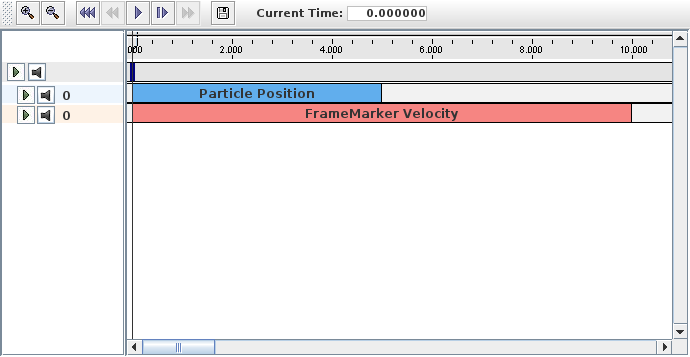
\includegraphics[]{images/timelineProbes}
\else
 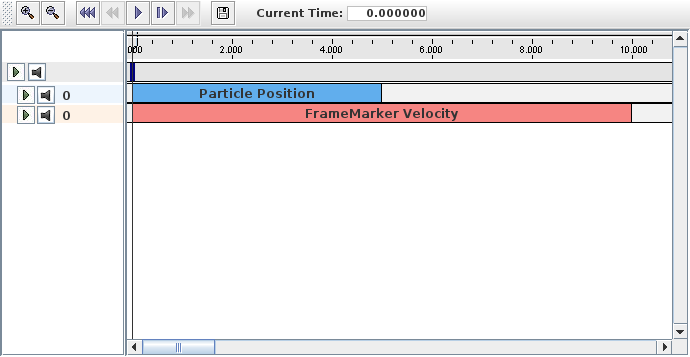
\includegraphics[width=4in]{images/timelineProbes}
\fi
\end{center}
\caption{Timeline view of the probes created by SimpleMuscleWithProbes.}
\label{probes:fig}
\end{figure}

\begin{figure}[ht]
\begin{center}
\iflatexml
 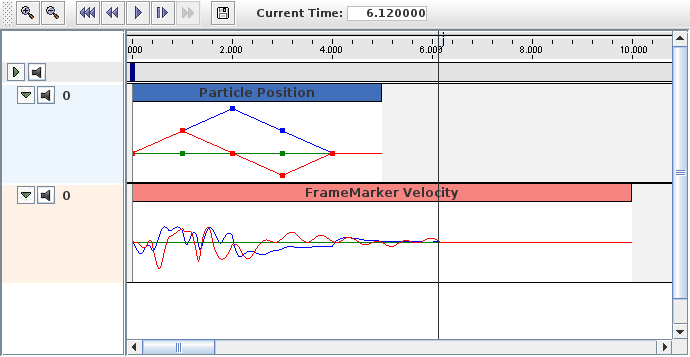
\includegraphics[]{images/timelineProbesExpanded}
\else
 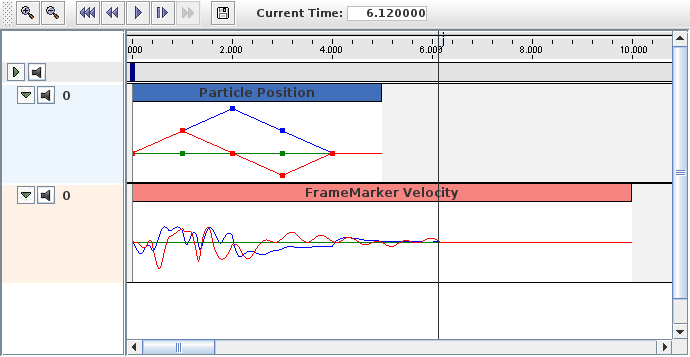
\includegraphics[width=4in]{images/timelineProbesExpanded}
\fi
\end{center}
\caption{Expanded view of the probes after {\tt
SimpleMuscleWithProbes} has run for about 6 seconds, showing the data
accumulated in the output probe {\tt "FrameMarker Velocity"}.}
\label{probesExpanded:fig}
\end{figure}

\subsection{Data file format}
\label{DataFileFormat:sec}

The data files associated with numeric probes are ASCII files
containing two lines of header information followed by a set of knot
points, one per line, defining the numeric data. The time value
(relative to the probe's start time) for each knot point can be
specified explicitly at the start of the each line, in which case the
file takes the following format:
%
\begin{lstlisting}[]
startTime stopTime scale
interpolation vsize explicit
t0 val00 val01 val02 ...
t1 val10 val11 val12 ...
t0 val20 val21 val22 ...
...
\end{lstlisting}
%
Knot point information begins on line 3, with each line being a
sequence of numbers giving the knot's time followed by $n$ values,
where $n$ is the vector size of the probe (i.e., the value returned by
{\tt getVsize()}).

Alternatively, time values can be implicitly specified starting at 0
(relative to the probe's start time) and incrementing by a uniform
{\tt timeStep}, in which case the file assumes a second format:
%
\begin{lstlisting}[]
startTime stopTime scale
interpolation vsize timeStep
val00 val01 val02 ...
val10 val11 val12 ...
val20 val21 val22 ...
...
\end{lstlisting}
%
For both formats, {\tt startTime}, {\tt startTime}, and {\tt scale}
are numbers giving the probe's start and stop time in seconds and {\tt
scale} gives the scale factor (which is typically 1.0).  {\tt
interpolation} is a word describing how the data should be
interpolated between knot points and is the string value of {\tt
Interpolation.Order} as described in Section
\ref{NumericProbeStructure:sec} (and which is typically {\tt Linear},
{\tt Parabolic}, or {\tt Cubic}). {\tt vsize} is an integer giving the
probe's vector size.

The last entry on the second line is either a number specifying a
(uniform) time step for the knot points, in which case the file
assumes the second format, or the keyword {\tt explicit}, in which
case the file assumes the first format.

As an example, the file used to specify data for the input probe in
the example of Section \ref{SimpleMuscleWithProbes:sec} looks like
the following:
%
\begin{lstlisting}[]
0 4.0 1.0
Linear 3 explicit
0.0  0.0 0.0 0.0 
1.0  0.5 0.0 0.5
2.0  0.0 0.0 1.0
3.0 -0.5 0.0 0.5
4.0  0.0 0.0 0.0
\end{lstlisting}
%
Since the data is uniformly spaced beginning at 0, it would also be
possible to specify this using the second file format:
%
\begin{lstlisting}[]
0 4.0 1.0
Linear 3 1.0
 0.0 0.0 0.0 
 0.5 0.0 0.5
 0.0 0.0 1.0
-0.5 0.0 0.5
 0.0 0.0 0.0
\end{lstlisting}
%

\subsection{Adding probe data in-line}

It is also possible to specify input probe data directly in code,
instead of reading it from a file. For this, one would use the
constructor
%
\begin{lstlisting}[]
   NumericInputProbe (ModelComponent c, String propPath, double t0, double t1);
\end{lstlisting}
%
which creates a {\tt NumericInputProbe} with the specified property
and with start and stop times indicated by {\tt t0} and {\tt t1}.
Data can then be added to this probe using the method
%
\begin{lstlisting}[]
   addData (double[] data, double timeStep);
\end{lstlisting}
%
where {\tt data} is an array of knot point data. This contains the
same knot point information as provided by a file (Section
\ref{DataFileFormat:sec}), arranged in row-major order.  Times values
for the knots are either implicitly specified, starting at 0 (relative
to the probe's start time) and increasing uniformly by the amount
specified by {\tt timeStep}, or are explicitly specified at the
beginning of each knot if {\tt timeStep} is set to the built-in
constant {\tt NumericInputProbe.EXPLICIT\_TIME}. The size of the {\tt
data} array should then be either $n*m$ (implicit time values) or
$(n+1)*m$ (explicit time values), where $n$ is the probe's vector size
and $m$ is the number of knots.

As an example, the data for the input probe in Section
\ref{SimpleMuscleWithProbes:sec} could have been specified
using the following code:
%
\begin{lstlisting}[]
      NumericInputProbe p1probe =
         new NumericInputProbe (
            mech, "particles/p1:targetPosition", 0, 5);
      p1probe.addData (
         new double[] {
            0.0,  0.0, 0.0, 0.0,
            1.0,  0.5, 0.0, 0.5,
            2.0,  0.0, 0.0, 1.0,
            3.0, -0.5, 0.0, 0.5,
            4.0,  0.0, 0.0, 0.0 },
            NumericInputProbe.EXPLICIT_TIME);
\end{lstlisting}

When specifying data in code, the interpolation defaults to {\tt
Linear} unless explicitly specified using {\tt
setInterpolationOrder()}, as in, for example:
%
\begin{lstlisting}[]
   probe.setInterpolationOrder (Order.Cubic);
\end{lstlisting}
%

\subsection{Numeric monitor probes}
\label{NumericMonitorProbes:sec}

In some cases, it may be useful for an application to deploy an output
probe in which the data, instead of being collected from various
component properties, is generated by a function within the probe
itself. This ability is provided by a
\javaclass[artisynth.core.probes]{NumericMonitorProbe}, which generates
data using its  \javamethodAlt{%
artisynth.core.probes.NumericMonitorProbe.generateData()}%
{generateData(vec,t,trel)}
method. This evaluates a vector-valued function of time at
either the absolute time {\tt t} or the probe-relative time {\tt trel}
and stores the result in the vector {\tt vec}, whose size equals the
vector size of the probe (as returned by
\javamethod[artisynth.core.probes.NumericProbeBase]{getVsize()}).  The
probe-relative time {\tt trel} is determined by
%
\begin{equation}
\text{trel} = (\text{t} - \text{tstart})/\text{scale}
\end{equation}
%
where {\tt tstart} and {\tt scale} are the probe's start time
and scale factors as returned by
\javamethod[artisynth.core.probes.Probe]{getStartTime()} and
\javamethod[artisynth.core.probes.Probe]{getScale()}.

As described further below, applications have several ways to control
how a {\tt NumericMonitorProbe} creates data:

\begin{itemize}

\item Provide the probe with a
\javaclass[artisynth.core.probes]{DataFunction} using the
\javamethodAlt{artisynth.core.probes.NumericMonitorProbe.setDataFunction()}%
{setDataFunction(func)} method;

\item Override the \javamethodAlt{%
artisynth.core.probes.NumericMonitorProbe.generateData()}%
{generateData(vec,t,trel)}
method;

\item Override the \javamethodAlt{%
artisynth.core.probes.NumericMonitorProbe.apply(double)}{apply(t)}
method.

\end{itemize}

The application is free to generate data in any desired way, and so in
this sense a {\tt NumericMonitorProbe} can be used similarly to a {\tt
Monitor}, with one of the main differences being that the data
generated by a {\tt NumericMonitorProbe} can be automatically displayed
in the ArtiSynth GUI or written to a file.

The \javaclass[artisynth.core.probes]{DataFunction} interface
declares an {\tt eval()} method,
%
\begin{verbatim}
   void eval (VectorNd vec, double t, double trel)
\end{verbatim}
%
that for 
{\tt NumericMonitorProbe}s
evaluates a vector-valued function of time,
where the arguments take the same role as for the monitor's \javamethodAlt{%
artisynth.core.probes.NumericMonitorProbe.generateData()}%
{generateData()}
method. Applications can declare an appropriate {\tt DataFunction} and
set or query it within the probe using the methods
%
\begin{lstlisting}[]
   void setDataFunction (DataFunction func);

   DataFunction getDataFunction();
\end{lstlisting}
%
The default implementation {\tt generateData()} checks to see
if a data function has been specified, and if so, uses that to
generate the probe data. Otherwise, if the probe's data function is {\tt
null}, the data is simply set to zero.

To create a {\tt NumericMonitorProbe} using a supplied {\tt DataFunction},
an application will create a generic probe instance, using one
of its constructors such as 
%
\begin{lstlisting}[]
   NumericMonitorProbe (vsize, fileName, startTime, stopTime, interval);
\end{lstlisting}
%
and then define and instantiate a {\tt DataFunction} and pass it to
the probe using {\tt setDataFunction()}. It is not necessary to supply
a file name (i.e., {\tt fileName} can be {\tt null}), but if one is
provided, then the probe's data can be saved to that file.

A complete example
of this is defined in
%
\begin{verbatim}
  artisynth.demos.tutorial.SinCosMonitorProbe
\end{verbatim}
%
the listing for which is:

\lstset{numbers=left}
\lstinputlisting{../../src/artisynth/demos/tutorial/SinCosMonitorProbe.java}
\lstset{numbers=none}

In this example, the {\tt DataFunction} is implemented using the class
{\tt SinCosFunction}, which also implements
\javaclass[maspack.util]{Clonable} and the associated {\tt clone()}
method. This means that the resulting probe will also be duplicatable
within the GUI. Alternatively, one could implement {\tt
SinCosFunction} by extending
\javaclass[artisynth.core.probes]{DataFunctionBase}, which implements
{\tt Clonable} by default. Probes containing {\tt DataFunction}s
which are {\it not} {\tt Clonable} will not be duplicatable.

When the example is run, the resulting probe output is shown in the
timeline image of Figure \ref{sinCosProbe:fig}.

\begin{figure}[ht]
\begin{center}
\iflatexml
 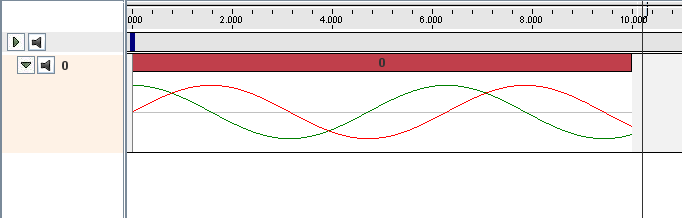
\includegraphics[]{images/sinCosProbe}
\else
 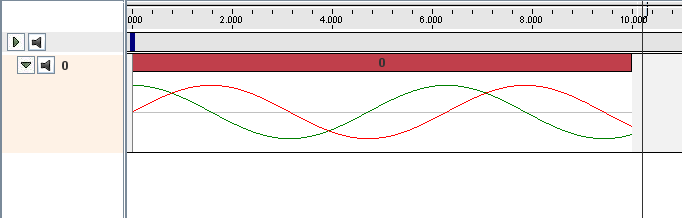
\includegraphics[width=4.5in]{images/sinCosProbe}
\fi
\end{center}
\caption{Output from a {\tt NumericMonitorProbe} which generates sine
and cosine waves.}
\label{sinCosProbe:fig}
\end{figure}

As an alternative to supplying a {\tt DataFunction} to a generic {\tt
NumericMonitorProbe}, an application can instead subclass {\tt
NumericMonitorProbe} and override either its \javamethodAlt{%
artisynth.core.probes.NumericMonitorProbe.generateData()}%
{generateData(vec,t,trel)} or \javamethodAlt{%
artisynth.core.probes.NumericMonitorProbe.apply(double)}{apply(t)}
methods. As an example of the former, one could create a subclass as
follows:
%
\begin{lstlisting}[]
  class SinCosProbe extends NumericMonitorProbe {
     
     public SinCosProbe (
        String fileName, double startTime, double stopTime, double interval) {
        super (2, fileName, startTime, stopTime, interval);
     }

     public void generateData (VectorNd vec, double t, double trel) {
        vec.set (0, Math.sin (t));
        vec.set (1, Math.cos (t));        
     }
  }
\end{lstlisting}
%
Note that when subclassing, one must also create constructor(s) for
that subclass. Also, {\tt NumericMonitorProbe}s which don't have a
{\tt DataFunction} set are considered to be clonable by default, which
means that the {\tt clone()} method may also need to be overridden if
cloning requires any special handling.

\subsection{Numeric control probes}
\label{NumericControlProbes:sec}

In other cases, it may be useful for an application to deploy an input
probe which takes numeric data, and instead of using it to modify
various component properties, instead calls an internal method to
directly modify the simulation in any way desired.  This ability is
provided by a \javaclass[artisynth.core.probes]{NumericControlProbe},
which applies its numeric data using its \javamethodAlt{%
artisynth.core.probes.NumericControlProbe.applyData()}%
{applyData(vec,t,trel)} method. This receives the numeric input data
via the vector {\tt vec} and uses it to modify the simulation for
either the absolute time {\tt t} or probe-relative time {\tt
trel}. The size of {\tt vec} equals the vector size of the probe (as
returned by
\javamethod[artisynth.core.probes.NumericProbeBase]{getVsize()}), and
the probe-relative time {\tt trel} is determined as described in
Section \ref{NumericMonitorProbes:sec}.

A {\tt NumericControlProbe} is the {\tt Controller} equivalent
of a {\tt NumericMonitorProbe}, as described in Section 
\ref{NumericMonitorProbes:sec}. Applications have several ways to control
how they apply their data:

\begin{itemize}

\item Provide the probe with a 
\javaclass[artisynth.core.probes]{DataFunction} using the
\javamethodAlt{artisynth.core.probes.NumericControlProbe.setDataFunction()}%
{setDataFunction(func)} method;

\item Override the \javamethodAlt{%
artisynth.core.probes.NumericControlProbe.applyData()}%
{applyData(vec,t,trel)}
method;

\item Override the \javamethodAlt{%
artisynth.core.probes.NumericControlProbe.apply(double)}{apply(t)}
method.

\end{itemize}

The application is free to apply data in any desired way, and so in
this sense a {\tt NumericControlProbe} can be used similarly to a
{\tt Controller}, with one of the main differences being that the
numeric data used can be automatically displayed in the ArtiSynth GUI
or read from a file.

The \javaclass[artisynth.core.probes]{DataFunction} interface
declares an {\tt eval()} method,
%
\begin{verbatim}
   void eval (VectorNd vec, double t, double trel)
\end{verbatim}
%
that for 
{\tt NumericControlProbe}s applies the numeric data, 
where the arguments take the same role as for the monitor's \javamethodAlt{%
artisynth.core.probes.NumericControlProbe.applyData()}%
{applyData()}
method. Applications can declare an appropriate {\tt DataFunction} and
set or query it within the probe using the methods
%
\begin{lstlisting}[]
   void setDataFunction (DataFunction func);

   DataFunction getDataFunction();
\end{lstlisting}
%
The default implementation {\tt applyData()} checks to see
if a data function has been specified, and if so, uses that to
apply the probe data. Otherwise, if the probe's data function is {\tt
null}, the data is simply ignored and the probe does nothing.

To create a {\tt NumericControlProbe} using a supplied {\tt DataFunction},
an application will create a generic probe instance, using one
of its constructors such as 
%
\begin{lstlisting}[]
   NumericControlProbe (vsize, data, startTime, stopTime, timeStep);

   NumericControlProbe (fileName);
\end{lstlisting}
%
and then define and instantiate a {\tt DataFunction} and pass it to
the probe using {\tt setDataFunction()}. The latter constructor
creates the probe and reads in both the data and timing information
from the specified file.

A complete example
of this is defined in
%
\begin{verbatim}
  artisynth.demos.tutorial.SpinControlProbe
\end{verbatim}
%
the listing for which is:

\lstset{numbers=left}
\lstinputlisting{../../src/artisynth/demos/tutorial/SpinControlProbe.java}
\lstset{numbers=none}

This example creates a simple box and then uses a {\tt
NumericControlProbe} to spin it about the $z$ axis, using a {\tt
DataFunction} implementation called {\tt SpinFunction}. A clone method
is also implemented to ensure that the probe will be duplicatable in
the GUI, as described in Section \ref{NumericMonitorProbes:sec}.  A
single channel of data is used to control the orientation angle of the
box about $z$, as shown in Figure \ref{spinControlProbe:fig}.

\begin{figure}[ht]
\begin{center}
\iflatexml
 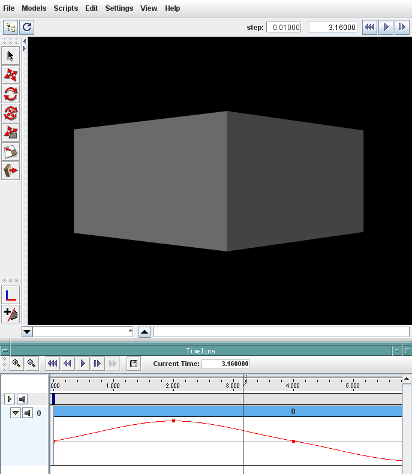
\includegraphics[]{images/spinControlProbe}
\else
 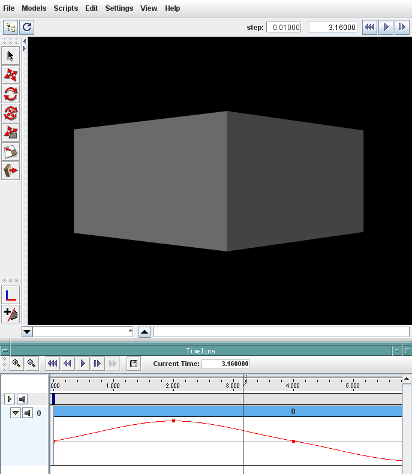
\includegraphics[width=4.5in]{images/spinControlProbe}
\fi
\end{center}
\caption{Screen shot of the {\tt SpinControlDemo}, showing the
numeric data in the timeline.}
\label{spinControlProbe:fig}
\end{figure}

Alternatively, an application can subclass {\tt NumericControlProbe}
and override either its \javamethodAlt{%
artisynth.core.probes.NumericControlProbe.applyData()}%
{applyData(vec,t,trel)} or \javamethodAlt{%
artisynth.core.probes.NumericControlProbe.apply(double)}{apply(t)}
methods, as described for {\tt NumericMonitorProbe}s (Section
\ref{NumericMonitorProbes:sec}).

\section{Application-Defined Menu Items}
\label{MenuItems:sec}

Application models can define custom {\it menu items} that appear
under the {\tt Application} menu in the main ArtiSynth menu bar.

This can be done by implementing the interface
\javaclass[artisynth.core.modelbase]{HasMenuItems} in either the {\tt
RootModel} or any of its top-level components (e.g., models,
controllers, probes, etc.). The interface contains a single
method
%
\begin{lstlisting}[]
   public boolean getMenuItems(List<Object> items);
\end{lstlisting}
%
which, if the component has menu items to add, should append them
to {\tt items} and return {\tt true}.

The {\tt RootModel} and all models derived from
\javaclass[artisynth.core.modelbase]{ModelBase} implement {\tt
HasMenuItems} by default, but with {\tt getMenuItems()} returning {\tt
false}. Models wishing to add menu items should override this default
declaration. Other component types, such as controllers, need to
explicitly implement {\tt HasMenuItems}.

\begin{sideblock}
Note: the {\sf Application} menu will only appear if {\tt getMenuItems()} returns
{\tt true} for either the {\tt RootModel} or one or more of its
top-level components.
\end{sideblock}

\javamethod*[artisynth.core.modelbase.HasMenuItems]{getMenuItems()}
will be called each time the {\sf Application} menu is selected, so the
menu itself is created on demand and can be varied to suite the
current system state. In general, it should return items that are
capable of being displayed inside a Swing {\tt JMenu}; other items
will be ignored. The most typical item is a Swing {\tt JMenuItem}.  The
convenience method
\javamethodAlt{maspack.widgets.GuiUtils.createMenuItem()}%
{createMenuItem(listener,text,toolTip)}
can be used to quickly create menu items, as in the following
code segment:
%
\begin{lstlisting}[]
   public boolean getMenuItems(List<Object> items) {
      items.add (GuiUtils.createMenuItem (this, "reset", ""));
      items.add (GuiUtils.createMenuItem (this, "add sphere", ""));
      items.add (GuiUtils.createMenuItem (this, "show flow", ""));
      return true;
   }
\end{lstlisting}
%
This creates three menu items, each with {\tt this} specified as an
{\tt ActionListener} and no tool-tip text, and appends them
to {\tt items}. They will then appear under the {\sf Application}
menu as shown in Figure \ref{applicationMenu:fig}.

\begin{figure}[t]
\begin{center}
\iflatexml
 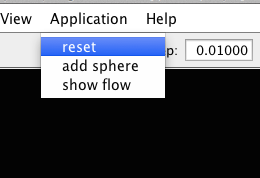
\includegraphics[]{images/applicationMenu}
\else
 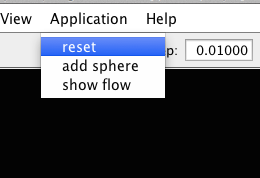
\includegraphics[width=2.5in]{images/applicationMenu}
\fi
\end{center}
\caption{Application-defined menu items appearing under the ArtiSynth
menu bar.}
\label{applicationMenu:fig}
\end{figure}

To actually execute the menu commands, the items returned by {\tt
getMenuItems()} need to be associated with an {\tt ActionListener}
(defined in {\tt java.awt.event}), which supplies the method {\tt
actionPerformed()} which is called when the menu item is
selected. Typically the {\tt ActionListener} is the component
implementing {\tt HasMenuItems}, as was assumed in the example
declaration of {\tt getMenuItems()} shown above. {\tt RootModel} and
other models derived from {\tt ModelBase} implement {\tt ActionListener} by
default, with an empty declaration of {\tt actionPerformed()} that
should be overridden as required.
A declaration of {\tt actionPerformed()} capable of handling the menu
example above might look like this:
%
\begin{lstlisting}[]
   public void actionPerformed (ActionEvent event) {
      String cmd = event.getActionCommand();
      if (cmd.equals ("reset")) {
         resetModel();
      }
      else if (cmd.equals ("add sphere")) {
         addSphere();
      }
      else if (cmd.equals ("show flow")) {
         showFlow();
      }
   }
\end{lstlisting}
%

%
